\documentclass[a4paper]{article}\usepackage[]{graphicx}\usepackage[]{color}
%% maxwidth is the original width if it is less than linewidth
%% otherwise use linewidth (to make sure the graphics do not exceed the margin)
\makeatletter
\def\maxwidth{ %
  \ifdim\Gin@nat@width>\linewidth
    \linewidth
  \else
    \Gin@nat@width
  \fi
}
\makeatother

\definecolor{fgcolor}{rgb}{0.345, 0.345, 0.345}
\newcommand{\hlnum}[1]{\textcolor[rgb]{0.686,0.059,0.569}{#1}}%
\newcommand{\hlstr}[1]{\textcolor[rgb]{0.192,0.494,0.8}{#1}}%
\newcommand{\hlcom}[1]{\textcolor[rgb]{0.678,0.584,0.686}{\textit{#1}}}%
\newcommand{\hlopt}[1]{\textcolor[rgb]{0,0,0}{#1}}%
\newcommand{\hlstd}[1]{\textcolor[rgb]{0.345,0.345,0.345}{#1}}%
\newcommand{\hlkwa}[1]{\textcolor[rgb]{0.161,0.373,0.58}{\textbf{#1}}}%
\newcommand{\hlkwb}[1]{\textcolor[rgb]{0.69,0.353,0.396}{#1}}%
\newcommand{\hlkwc}[1]{\textcolor[rgb]{0.333,0.667,0.333}{#1}}%
\newcommand{\hlkwd}[1]{\textcolor[rgb]{0.737,0.353,0.396}{\textbf{#1}}}%

\usepackage{framed}
\makeatletter
\newenvironment{kframe}{%
 \def\at@end@of@kframe{}%
 \ifinner\ifhmode%
  \def\at@end@of@kframe{\end{minipage}}%
  \begin{minipage}{\columnwidth}%
 \fi\fi%
 \def\FrameCommand##1{\hskip\@totalleftmargin \hskip-\fboxsep
 \colorbox{shadecolor}{##1}\hskip-\fboxsep
     % There is no \\@totalrightmargin, so:
     \hskip-\linewidth \hskip-\@totalleftmargin \hskip\columnwidth}%
 \MakeFramed {\advance\hsize-\width
   \@totalleftmargin\z@ \linewidth\hsize
   \@setminipage}}%
 {\par\unskip\endMakeFramed%
 \at@end@of@kframe}
\makeatother

\definecolor{shadecolor}{rgb}{.97, .97, .97}
\definecolor{messagecolor}{rgb}{0, 0, 0}
\definecolor{warningcolor}{rgb}{1, 0, 1}
\definecolor{errorcolor}{rgb}{1, 0, 0}
\newenvironment{knitrout}{}{} % an empty environment to be redefined in TeX

\usepackage{alltt}
\usepackage{fullpage}
\usepackage{setspace}
    \doublespacing
%\usepackage[usenames,dvipsnames]{xcolor}
\usepackage{hyperref}
\hypersetup{
    colorlinks,
    citecolor=black,
    filecolor=black,
    linkcolor=blue,
    urlcolor=blue
}
\usepackage{dcolumn}
\usepackage{booktabs}
\usepackage{url}
\usepackage{tikz}
\usepackage{todonotes}
\usepackage[T2A]{fontenc}
\usepackage[utf8]{inputenc}
\usepackage[english]{babel}
\usepackage{graphicx}

\usepackage{csquotes}
\usepackage[style=authoryear, sorting=ynt, backend=bibtex]{biblatex}
\addbibresource{mybib.bib}
\IfFileExists{upquote.sty}{\usepackage{upquote}}{}

\begin{document}





\title{Why are the Most Trade-Open Countries More Likely to Repress the Media?}

\author{Justin Murphy}

\maketitle

\begin{singlespace}
\begin{abstract}
Why are more trade-open countries more likely to repress the media, even though media freedom is positively correlated with most other components of economic globalization? To explore and understand this little-known empirical puzzle, I argue that economic globalization exerts contradictory pressures on state-media relations. On the one hand, economic openness encourages national policymakers to promote media freedom because foreign investors are more likely to invest where information is reliable. On the other hand, because adjusting to economic openness implies distributive conflict which can threaten the government, openness also generates incentives for national policymakers to suppress information and communication about the costs of liberalization. This paper develops a theoretical model that reconciles these contradictory expectations by disaggregating economic globalization into its component parts and distinguishing changes (liberalization) from levels of economic globalization (openness). I argue that liberalization of trade, inward foreign direct investment, and inward capital flows increase the probability states will repress the media, as states seek to quell domestic conflict around the adjustment costs of liberalization. In the long run, however, different types of economic openness exert different pressures on media freedom depending on how much they reward transparency. I argue that financial openness leads to greater media freedom in the long run because transparency is important to capital markets, but trade openness exerts no positive effect on media freedom in the long run because foreign importers and exporters are unaffected by transparency in other countries. To test these expectations, I use a mixed-methods research design employing large-N statistical tests combined with process-tracing in Argentina and Mexico.
\end{abstract}
\end{singlespace}

\vspace{0.3cm}

Given the conventional wisdom that democratic political institutions drive economic openness \parencite{Milner:2005ci} and vice-versa \parencite{EICHENGREEN:2008gg}, it is surprising that since the 1960s, on average, those countries which have been more open to international trade have had lower levels of media freedom. Although international portfolio capital and foreign direct investment are each positively correlated with media freedom around the world, the bivariate relationship between trade and media freedom is slightly negative.Disaggregated economic data come from the World Bank Development Indicators (Bank 2012) and data on media freedom come from Freedom House () and Van Belle's Global Press Freedom Dataset (Van Belle 2000). See the section on Data and Method below for a more detailed discussion of data and coding. Considering the 151 countries between 1960 and 2011 for which there is available data, those countries which most often had a repressive media environment had higher levels of trade than those countries which most often had a free media. This is true in democratic and non-democratic countries, although the negative relationship is weaker in democratic countries. Given the positive correlation found between media freedom and other measures of economic openness such as portfolio capital flows foreign direct investment, and the KOF Globalization index (Dreher et al. 2008), the coincidence of high trade openness and media repression is a surprisingly under-reported empirical puzzle in international and comparative political economy.

\pagebreak
\begin{figure}[t]
    \caption{Trade vs. General Economic Globalization in the Politics of Media Freedom, 1970-2003}
    \label{absolute}
    \begin{center}

\begin{knitrout}
\definecolor{shadecolor}{rgb}{0.969, 0.969, 0.969}\color{fgcolor}

{\centering 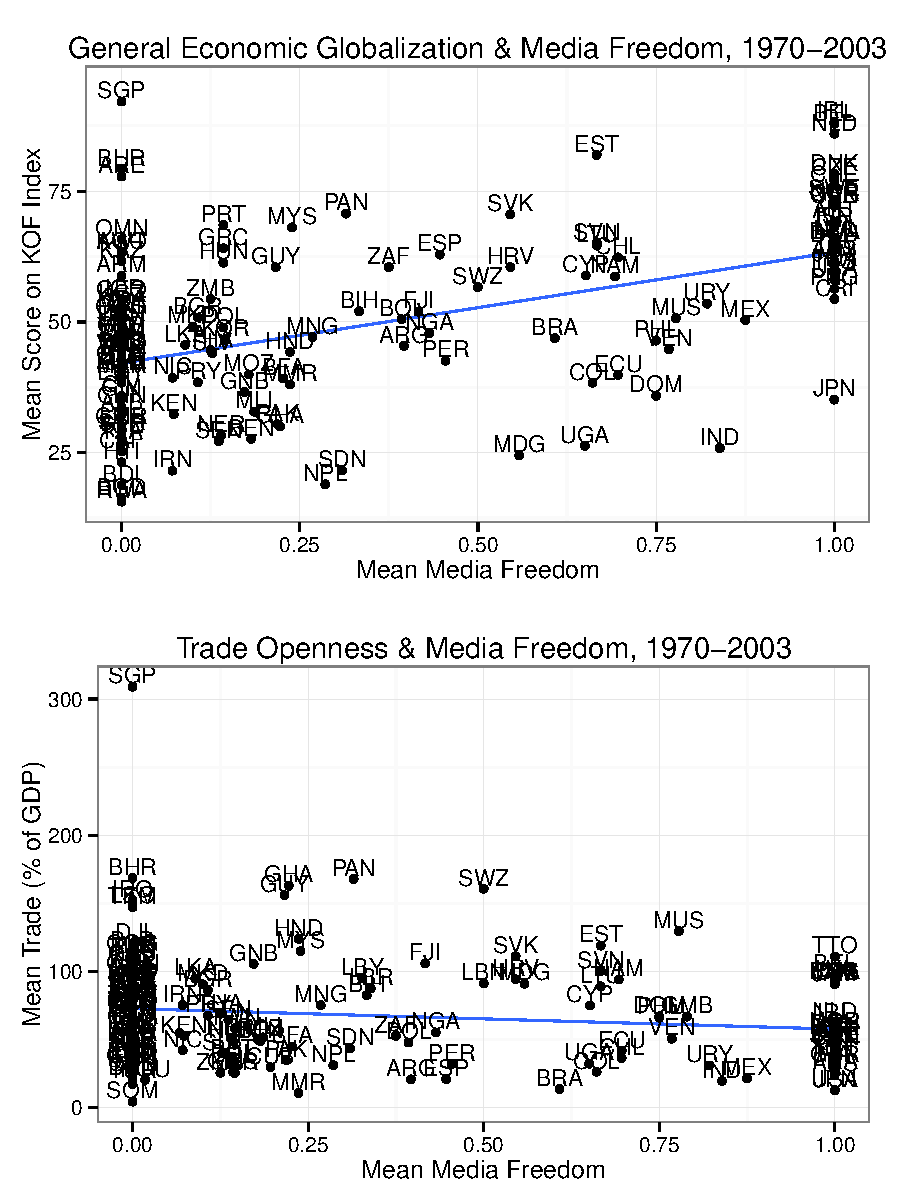
\includegraphics[width=0.8\linewidth]{figures/intrographs} 

}



\end{knitrout}


    \end{center}
    \begin{singlespace}
        {\scriptsize{The KOF Index of Globalization is a 100-point scale reflecting the quantity of international trade and investment policy restrictions as well as flows of trade, FDI, FPI, and income paid to foreign nationals and capital (Dreher et al 2008, 43). Media freedom is measured on a dichotomous scale (free or not free). See the section on Data and Method for more details. 
                      }}
    \end{singlespace}
\end{figure}

This puzzle points to a larger gap in research on the domestic effects of economic globalization. International and comparative political economists have not yet developed a serious theoretical and empirical account of how a country's media are likely to be affected by that country's integration into the international economy. Much is known about the effects of economic integration on aspects of domestic politics such as cleavages (Rogowski 1987, 1989; Hiscox 2002), growth rates (Rodriguez and Rodrik 2001); domestic spending (Rodrik 1998; Burgoon 2001), civil war (Barbieri and Reuveny 2005; Bussmann and Schneider 2007), and generic measures of democracy (Eichengreen and Leblang 2008; Li and Reuveny 2003), but very little is known about how economic integration affects state-media relations. One exception is a working paper by Orion Lewis (2008), which finds mixed but suggestive evidence that trade openness is negatively related to media freedom and portfolio capital is positively related to media freedom. Other research has considered whether political and civil liberties (broadly including freedom of the media) affect international economic flows (2007) and the effect of media in economic reform (Coyne and Leeson 2004; Islam 2002), but in the extant literature there is no systematic analysis of whether and in what ways domestic media freedom has been shaped by increasing international economic integration around the world.

\section{Globalization, Democracy, and Media}

The present study provides a theoretical account of how different international economic flows affect domestic media freedom differently, focusing on the puzzling negative correlation between trade levels and media freedom. It improves on the limited previous research in two ways. First, Lewis (2008) uses only the Freedom House measures of press freedom and therefore considers country-level panel data only between 1993 and 2006. The present study incorporates the Global Media Freedom Index by Van Belle (2000; 1997) to consider a similar panel of countries for the much longer timeframe from 1948 to 2009. Second, I emphasize the difference between levels and changes (long-run and short-run effects) in a country's exposure to international economic flows, whereas Lewis considers only levels.

Previous research provides strong reasons to expect the global integration of markets to exert pressures on institutions of democracy, but there remains much theoretical uncertainty about the degree to which these effects are positive or negative. Many have argued that economic globalization generates economic growth which strengthens democratic institutions (Baghwati 1997; Im 1996), increases incentives for peace (Baghwati 1997; Oneal and Russett 1999), or diffuses democracy as a norm (Kant 1983; Limongi et al. 1996) On the other hand, many have argued that economic globalization is negatively associated with democracy because it rewards efficiency rather than popular sovereignty (Dominguez and Huntington 1975; Lindblom 1977; Cammack 1998), or because leaders may prefer to repress rather than compensate the domestic losers from increased openness (Adserà and Boix 2002).See Li and Reuveny 2003 for a detailed overview of this debate. Within the general debate surrounding the globalization-democracy nexus, some researchers such as Li and Reveuny (2003) have sought greater clarity by disaggregating the distinct types of international economic flows and considering them separately, but relying on standard aggregate measures of democracy. Li and Reveuny find that trade and portfolio capital have negative effects on democracy, while foreign direct investment and democratic norms have a positive effect, but their dependent variable of democracy is calculated with the common procedure of subtracting the Polity autocracy score from the Polity democracy score. Thus, despite much research on the relationship between economic globalization and democracy, and despite evidence that disaggregation is fruitful for understanding this nexus of relationships, relatively little is known about how different international economic flows affect the various institutions which separately constitute what we know as democracy.

In particular, very little research to date queries whether and how economic globalization shapes state policies regarding domestic media freedom. One exception is Lewis (2008), who finds that FDI inflows are positively associated with press freedom, trade levels are negatively associated with media freedom, and portfolio capital inflows have no discernible effect on press freedom. But as a first investigation into this question and as a largely inductive effort to establish the statistical patterns, the theoretical interpretations of this article are mostly provisional. Additionally, Lewis considers only levels of trade and year-by-year inflows of FDI and portfolio capital, whereas recent research shows that the distinction between flows (year-to-year movements) and stocks (the sum of all previous flows) is crucial in researching the effects of foreign investment on repression (2012). As discussed above, Antonis and Fillapaois (2007) consider the effect of civil liberties such as media freedom on FDI, but not whether FDI affects civil liberties.

However, previous research on the relationship between markets and media more generally provides a basis for theorizing the relationship between economic integration and media freedom. Broadly, one tradition argues that the spread of markets and freer media are positively associated (Habermas 1991; Islam 2002; Islam 2003). However, an opposite tradition suggets that markets and the logic of profits and efficiency create incentives for authoritarianism (Dominguez and Huntington 1975). With respect to media politics in particular, Gehlbach and Sonin (2011) show that larger advertising markets are associated with nationalization of private media because, they argue, the benefits of state control increase with the advertising market. If economic liberalization tends to enlarge advertising markets by spurring economic growth, then liberalization might increase the state's incentives to repress private media just as it increases incentives to nationalize it. Furthermore, international economic integration brings the threat of social and political backlashes (Bussmann and Schneider 2007), which require the state to compensate the domestic losers from globalization (Rodrik 1998) or, alternatively, repress them (Adserà and Boix 2002).

On the other hand, the literature on 'competitive authoritarianism' suggests that increasing economic interdependence is one of the forces which has increasingly rendered traditional authoritarian repression unfeasible (Levitsky and Way 2002, 60, 62). As a country becomes increasingly integrated with the world economy, it increases the costs of overt authoritarianism by increasing the salience of international opinion, increasing the voice of domestic opposition, and increasing the number of domestic actors affected by international perceptions (Levitsky and Way 2006). For example, Fujimori in Peru in 1992 and Putin in Russia in 1993 failed in their efforts to overtly circumvent the legislature in part due to such international pressures (Levitsky and Way 2002, 56). International pressures against overt authoritarianism force regimes to adopt formally democratic institutions such as elections, but often leaves them free to violate human rights and civil liberties. For example, in the US-Mexico negotiations leading up to the North-American Free Trade Agreement, Mexican leaders made significant changes to present a front of democracy and respect for human rights to encourage investors, but there was no specific or formal conditionality which would have prohibited or even discouraged the repression of civil liberties if necessary.

At the same time, Levitsky and Way highlight the media as one of the four main arenas in which incumbent governments can contest and subvert international pressures to democratize. Competitive authoritarian governments may permit a formally independent and relatively free media, as in Peru, Serbia, Panama, or Nicaragua during the late 1980s and much of the 1990s, while engaging in alternative, more subtle tactics of repression, such as manipulative adminstrations of the law or tax code (Levitsky and Way 2002, 53,58)

While economic integration engenders distributive conflicts which tempt states to repress certain domestic groups at the same time it disincentivizes certain overt techniques of repression, governments around the world increasingly engage in strategic, authoritarian interventions into domestic media politics. Corrales and Westhoff (2006) find, for instance, that authoritarian regimes are more likely to develop television than internet, because television is more easily controlled. Additionally, many authoritarian regimes welcome the internet but are actively pursuing techniques of information control and manipulation on the internet in a networked fashion (MacKinnon 2011; Pearce and Kendzior 2012). These findings show that however much economic integration is making certain forms of repression obsolete, newer and more subtle techniques of media repression remain both attractive and viable.

As Antonis and Fillapaois point out, and as Lewis also argues, research on the relationship between globalization and democratic institutions likely shows such contradictory results because different international economic flows exert different pressures. To build on this idea while advancing the literature beyond the limitations discussed above, the next section provides a more deductive account of preicisely why we should expect various types of international economic openness to exert different effects on media freedom.

\section{Theory and Hypotheses}

Based on the review of previous research regarding the domestic political effects of international economic flows and the media politics of competitive authoritarianism, I develop a simple, informal rational-choice model of how state media policy should respond to trade, foreign direct investment, and portfolio capital flows. Consider a state which experiences a variable increase in some inward, international economic flow of trade, FDI, or portfolio capital. This increased flow will increase the income of certain domestic groups and decrease the income of others, according to well-developed open-economy expectations. The increased economic flow can be thought of as random and exogenous or the result of conscious state policy such as lowering tariffs. If they are well-informed and mobilized, a domestic group which experiences a negative income shock from economic liberalization would demand that the policymaker either close the domestic economy or compensate the group for its income loss, or else face rebellion. The “rebellion” could be electoral if the state is a democracy or a violent insurgency if the state does not have institutions to facilitate peaceful change. After experiencing the international shock, the media, if free to do so, would report the protests of the aggrieved group and its causes, namely, increased national exposure to the international economy and its conflictual distributive consequences. However, if the media does not fully report the political context and consequences of the international shock, the group which suffered an income loss would not threaten rebellion at all. A free media, in other words, are essential for domestic losers from globalization to exercise power in the domestic politics around the distributive outcomes of economic globalization. Where there is a free media, domestic losers from globalization hold policymakers accountable, but where there the media are manipulated by government, the claims of aggreived groups cannot exact concessions from holding policymakers accountable. This can be from either not reporting and therefore not informing domestic groups of the political-conflictual nature of globalization, or from silencing those claims if and when they are made.

After increased exposure occurs, the policymaker would prefer not to compensate the domestic group but prefers compensation to facing rebellion or closing the economy to ex ante levels. The policymaker can close the political process to any competitors to obviate the political pressure to compensate them (Adserà and Boix 2002), but the higher their level of integration, the more costly are overt types of repression (Levitsky and Way 2002). Supposing that a policymaker can choose among compensating the aggrieved domestic group, excluding competitors from the political process, or engaging in some repressive practices which vary on a continuum from overt to covert. In effect, we can conceptualize their utility function as including a penalty on overtness which increases with the country's economic integration, such that there is decreasing utility to overt forms of repression such as outright exclusion from the political process or government killings but this disutility approaches zero for repressive tactics which are relatively obscure such as the selective prosecution or financial targeting of opponents.

Among the less visible ways of exercising anti-democratic control, information-communication control will be uniquely attractive for the policymaker. This is because not only are repressive media tactics less severe than mass killings or canceling elections, but because control of the media could potentially tame international judgments independently by shaping what gets reported internationally. That is, control of the media can first minimize policymaker accountability for the adjustment costs of liberalization by suppressing domestic dissent, but policymakers could also reasonably expect that suppressing information at home would decrease the flow of negative information abroad, promoting their international image in part by repressively shaping their image at home. In summary, increasing linkages to other states and international pressures raise the cost of overt repression for liberalizing states, which increases the attractiveness of more subtle, lower-visibility tactics for suppressing dissent against liberalization. Repression of the media stands out as a uniquely attractive first because it is precisely such a relatively low-visibility, low-salience type of repression but also because if successful it would tend to lower negative visibility in general.

\subsection{Differences among trade, foreign direct investment, and portfolio capital}

The previous subsection argues that media repression is uniquely attractive to incumbents presiding over economic liberalization. However, the international actors who are the counterparties to a country's international exchanges are also strategic actors. When a government represses the flow of information and communication within its territory, these counterparties will respond strategically depending on how their particular investment in the country is affected by domestic freedom of information and communication. Given that these international counterparties have very different stakes in domestic media freedom depending on whether they are engaged in trade, foreign direct investment, or portfolio capital investment, the utility of media repression during economic liberalization will be conditioned according to a country's composition of exposure to these flows.

\subsection{Foreign Direct Investment}

FDI is defined as the private capital flows from one firm to an enterprise located in a country outside of the firm's home nation. FDI flows consist of equity capital, intercompany debt, and reinvested earnings, whenever the investment is sufficient to give the firm a controlling stake (typically 10\%) in the enterprise (Group 2004, 9: Jensen 2003, 588) Foreign direct investment is unique among other types of international investment in that FDI involves a longer-term committment and thus the interests of FDI investors are relatively more aligned with the long-term interests of host countries (Lipsey 1999; Jensen 2003, 588). The standard economic theory of FDI suggests that firm-level investment decisions to invest directly in a foreign country are not based on relative factor endowments or comparative rates of return, but on domestic market imperfections which can be exploited by multinational corporations (MNCs) better than domestic firms (Hymer 1960; Dunning 2013). The distributive consequences of FDI inflows are complex: FDI is typically thought to increase inequality between skilled and unskilled workers as MNCs tend to be technologically skill-biased relative to domestic firms (Feenstra and Hanson 1997) and unskilled, subsistence farmers do not have the resources to become entrepreneurs (Basu and Guariglia 2007). However, FDI is also thought to decrease overall domestic income inequality as an increase in the supply of capital relative to labor increases wages and reduces inequality between capital and skilled labor (Jensen and Rosas 2007). Jensen and Rosas present evidence that, because poor countries have relatively little skilled labor, FDI's effect on closing the gap between skilled labor and capital is likely to decrease inequality on net even if it increases inequality between skilled and unskilled labor. Thus, FDI inflows generate distributive conflict among skilled and unskilled labor, but are unlikely to generate highly salient distributive conflict overall. This expectation is borne out by research on the relationship between economic globalization and civil war. Bussmann and Schneider (2007) find, contrary to their expectations, that inflows of FDI decrease rather than increase the likelihood of civil war onset.

Most significantly, of the three types of international economic actors considered here, investors of FDI have a long-term stake in the conditions of a host country. Because of this, despite long-standing expectations that foreign direct investors prefer the efficiency of authoritarian regimes, the balance of evidence suggests that democracies draw greater FDI flows than autocracies because they are more credible (Jensen 2003, 588). Some scholars have sought to extend this logic by arguing that FDI should be attracted to respect for human rights (Blanton and Blanton 2007) have faced problems of measurement and missing data (Sorens and Ruger 2012). After accounting for these issues, Sorens and Ruger find no link between FDI and human rights. Thus, while formal democracy attracts FDI and FDI does not appear to generate intense distributive conflicts, neither does it appear to “punish” governments for violating human rights.

Interestingly, Antonis and Filipaios find, consistent with Jensen, that FDI seeks strong political rights while its attraction to civil rights is hump-shaped such that FDI is associated with both high and low levels of civil rights (2007). One possible explanation of these inconsistencies is that the socially positive consequences of FDI (rewarding democracy and rule of law and decreasing civil war onset) occur at the same time as, or perhaps in part through, the repression of civil rights. This is consistent with the model presented above, wherein the repression of a particular civil right (the freedom of expression) embodied in media freedom is repressed to dampen the disruptive effects of new FDI inflows, but in the long run equilibriates to a high level alongside political rights.

Thus, as argued in the previous section, increases in FDI should be associated with media repression, but in the long run FDI should be associated with media freedom. Because FDI is not averse to violations of rights per se, and is perhaps attracted to governments with low respect for civil rights, governments will use media repression to suppress distributive conflicts associated with FDI, but after the adjustment takes place and threat of conflict subsides, then FDI in the long-run should be associated with media freedom for the same reasons it is associated with democracy, namely credibility and stability.

\subsection{Portfolio capital}

Portfolio capital is defined as the purchase of stocks and bonds of less than 10\% of the outstanding stock of foreign firms (Kenen 1994, Walther 1997). The standard economic theory is that portfolio capital tends to flow where the rate of return on the target country's domestic assets is high relative to the riskiness of the investment (Mosley 2003, 743; Ahlquist 2006, 685). Portfolio capital is distinguished by its short-term, speculative nature compared to FDI. In a benchmark study of how portfolio investors evaluate political risks, Bernhard and Leblang (2002) show that portfolio investors respond to changes in country's political system (such as elections), but not to the substance of those changes (for instance, partisanship). Brooks and Mosley (2007) show that portfolio investors do respond to the substance of policymaking, such as partisanship and macroeconomic priorities, but only in low-information environments such as electoral turnovers. The effects of partisanship and macroeconomic policy on portfolio capital decrease when the political system itself is stable. The overall point is that portfolio investors are first and foremost interested in stability and predictability rather than particular policies, which only matter in periods when the predictability of the future is low.

Portfolio capital inflows tend to appreciate the domestic currency, which makes imports relatively cheaper in the home market and exports relatively more expensive to foreigners. This will harm exports, leading possibly to unemployment or decreases in wage levels in export-intensive industries. It will also make it harder for domestic firms to compete with relatively cheaper imports, also possibly leading to unemployment or wage decreases. Finally, cheaper capital imports can encourage skill-biased shifts in technology usage, increasing the incomes of skilled labor and decreasing the incomes of unskilled labor (Cragg et al. 1996; Ros and Lustig 2000). Finally, because portfolio capital is relatively liquid, the threat of sudden withdrawal by international investors is well-known to have highly negative macroeconomic effects, such as in Mexico in 1995 and Argentina in 2001.

Given the interests of governments and portfolio investors, governments should be inclined to repress the media in response to the distributive effects of portfolio capital for two reasons. First, inflows of portfolio capital will make governments more beholden to the prevention of systemic political risks such as general strikes, expropriations, or revolutions (Clark 1997). This is consistent with anecdotal evidence of portfolio investors who prefer governments to repress social unrest. Neoliberal economic reforms including international liberalization are often followed by large increases in foreign portfolio capital, and there is anecdotal evidence that in some cases foreign investors demand repression explicitly, such as when Chase Bank's Emerging Markets Group circulated a memo urging Mexican President Ernesto Zedillo to “eliminate the Zapatistas” and their uprising in Chiapas in 1994 (Silverstein and Cockburn 1995). Second, given that policy is evaluated by foreign investors largely in light of what is already known about the government and its history, incumbents who preside over financial liberalization for that very reason are likely to be sufficiently trusted by foreign capital that relatively subtle tactics such as media repression would be unlikely to shake confidence, especially if it is in the interest of preventing larger disruptions such as rebellions. It may be objected that portfolio investors would dislike media repression because they rely on a reliable flow of information regarding the country's conditions, but through modern “news management” politicians can practice a highly nuanced kind of transparency for international observers and also seek to repress domestic media using underhanded tactics. Indeed, country's which are open enough to receive capital inflows are likely to already be relatively transparent in the ways most relevant to investors, and this transparency required to induce investment might even embolden the assertiveness of domestic media.This appeared to happen in Mexico during the 1980s and 90s (Lawson 2002) Portfolio investors can typically rely on international news sources which are less likely to be targeted within the host country (on account of their financial independence and being linked to another sovereign, such as that one in Argentina). Finally, portfolio investors often have access to private, elite channels which provide them with politically important information about foreign country conditions before it would even be reported by free media (Dube et al. (2011)).

Thus, we should expect media policy to respond to inflows of portfolio capital just as it responds to FDI inflows. As a country adjusts to the destabilizing distributive effects of international portfolio investment, governments will be more likely to repress the media as a relatively discreet tactic of pacifying social unrest, consistent with investors' interests in stability. However, inflows of portfolio capital will in the long-run be associated with media freedom, as portfolio investors prefer high-information environments ceteris paribus.

\subsection{Trade}

Trade, defined simply as imports plus exports as the percentage of a country's gross domestic product, is unique among the previous two components of economic globalization in that the international counterparties have no direct economic stake in the social and political conditions of the home country. Put simply, trade is not an investment as are FDI and portfolio capital flows. The standard economic intuition explaining trade flows, although many sophisticated variations and extensions have been developed, is still the well-known Ricardian theory of comparative advantage. Other things equal, countries will tend to specialize in producing for export those goods which they are most advantaged in producing, and import from foreign producers those goods which domestic producers are unable to produce as efficiently.

International trade theory and much research in political science provides well-established expectations regarding the distributive effects of a country increasing its exposure to international trade. The standard Stolper-Samuelson model (1941) expects that increasing trade openness increases the income of the domestically abundant factor while decreasing the income of the domestically scarce factor. Thus, in capital-rich countries (industrialized or post-industrial countries), increasing trade openness benefits capital and harms labor, whereas in capital-poor countries increasing trade openness is expected to benefit labor and harm capital owners. In his benchmark study on the political consequences of these distributive expectations, Rogowski (1989) finds strong evidence that domestic political coalitions are empowered and disempowered by international trade as the Stolper-Samuelson model predicts. Hiscox (2002) further refines these expectations by showing that history is more finely explained by distinguishing the relative mobility of factors: when domestic factors are relatively immobile within the domestic economy, we do not observe class-based cleavages but rather sector-based cleavages and cross-class alliances, as immobility weds the interests of labor and capital to their shared industry. In turn, the threat of distributive conflict from international trade has been found salient enough to explain domestic political outcomes as diverse as the size of welfare states (Cameron 1978; Burgoon 2001) and the onset of civil wars (Bussmann and Schneider 2007).

The international counterparties to a country's international trade have a uniquely low stake in the political stability of the country, for the simple reason that the import and export of goods and services is not directly affected by the sanctity of civil rights such as freedom of expression or media freedom. Although emerging international norms of “corporate responsibility” and “fair trade” are increasingly visible in marketing for consumers in the wealthy democracies, these norms revolve around specific labor market issues such as child labor, “sweatshops”, and wages paid to workers in developing countries (Moore 2004). Even if some consumers in the wealthy democracies are increasingly willing to pay for more humane production conditions in foreign countries (effectively an international tax on repressive production conditions), there is no evidence and little reason to believe that economic behavior in importing or exporting goods and services anywhere in the world is in any way responsive to the sanctity of significantly less salient civil rights such as media freedom. For instance, consumers in the global North may very well prefer to pay premiums for coffee explicitly labeled as “fair trade,” but this provides no reason to expect they would pay more or less depending on whether the exporting country's trade agreements were facilitated by media repression. Similarly, if exporters in one country benefit from lowered tarrifs in a foreign country, compared to FDI and portfolio investors, they have uniquely less at stake in the political consequences faced by the foreign country with rising imports.

Thus, as with FDI and portfolio capital, we expect changes in trade openness to be associated with a higher probability of media repression, but unlike FDI and portfolio capital, we expect this effect of trade liberalization to persist into the long run, as governments face no pressure from their counterparties to eventually transition to a free media environment. If true, this would explain the puzzlingly negative correlation between international trade and media freedom despite the positive association between trade and most other components of economic globalization.

\subsection{Summary of Hypotheses}

To summarize, the hypotheses of the preceding subsections can be stated concisely as follows.

H1: Levels of trade openness decrease media freedom.

H2. Levels of portfolio capital increase media freedom.

H3. Levels of foreign direct investment increase media freedom.

H4. Changes in trade, equity, and FDI decrease media freedom.

\section{Data, Method, and Strategy}

To assess the theory, this article pursues a mixed-method research design employing large-N statistical tests and qualitative within-case analysis on two historically important cases. The intuition behind this research strategy is that statistical analyses are necessary to disentangle the independent effects of each economic flow, especially in distinguishing between short-run and long-run effects, while qualitative analysis is necessary for establishing the existence of a causal process.

In the quantitative analyses, I use state-level economic data collected by Sorens and Ruger (2012) for the main independent variables of interest (FDI, portfolio capital, and trade) for all available countries between 1948 and 2010. For the dependent variable, I use the well-known Freedom of the Press scores from Freedom House (CITATION) as well as the the Global Media Freedom Database (Van Belle 1997; 2000). Freedom House measures press freedom on a continuous scale from 0 to 100 and covers most countries from 1994 to the end of the economic time-series, whereas Van Belle's data is essentially a dichotomous measure of media freedom (footnote: it reduces to that) and covers most countries from 1948 to 1995. To maximize the sample, I create a single measure of press freedom which converts the Freedom House scores for 1994-2010 to Van Belle's dichotomous scale by interpolating from the two years for which there are observations on both measures.Specifically, I fit a logistic regression of the dichotomous variable on the continuous variable for the three years of overlapping observations, 1994-1996. Then for each year post-1995, I imputed to each each country a 1 on the dichotomous scale for each year their value on the continuous scale had greater than or equal to a .5 probability of being classified by the model as 1 (roughly all values greater than about 61 on the 100-point scale), and I gave them a 0 otherwise. This operation is somewhat inefficient (information is lost from the continuous measure) and biased (for some countries it generates artificial “changes” in value between the two time periods) but it credibly and consistently extends the time series for most countries and represents the most spatially and temporally extensive single measure of media freedom available. Thus, I employ it for the primary analyses but then model and account for possible spurious “effects” due to this operation. To distinguish the separate effects of different economic flows on media freedom across countries and over time, I use a series of cross-sectional time-series regression techniques and robustness checks, including panel vectorautoregression to check against reverse causality.

To corroborate the quantitative findings and enhance our understanding of the key puzzle motivating this paper, a following section offers two within-case analyses which trace the process whereby trade liberalization exerts pressure on domestic media freedom. To help control for confounding spatial and temporal factors, I consider two "third-wave" democracies from the same region in the same time period, Argentina and Mexico in the period between 1990 and 2011. These countries are analytically well-suited for further examination because they both democratized beginning in the 1980s and were consolidating in the 1990s. In autocratic regimes, even if we observed instances where media repression follows economic liberalization, it would be hard to infer that liberalization caused media repression because the media repression could be a function of auotcracy in general. On the other hand, if media repression follows economic liberalization in countries which are otherwise politically liberalizing, it will be more credible to infer that possibly economic liberalization generated the tendency to media repression. Indeed, Argentina and Mexico are least likely cases to expect media repression at this time because Argentina's Carlos Menem and Mexico's Carlos Salinas were championed by American politicians as models of democratic economic liberalization. Latin America is also a substantively attractive region for further study because Latin America is typically considered the first region where democracies were able to implement politically difficult "stabilization" policies. In the 1970s, it was a puzzle how economic liberalization would ever be achieved in democratic settings, given the status quo bias of elected politicians and the popular support for protectionist policies. An implication of this paper's argument, however, is that even in formally democratic countries economic liberalization may in some cases induce anti-democratic tactics such as media repression. If this is argument is correct, then substantively it would be most rewarding to better understand these cases which the conventional wisdom holds to be democratic sucess stories. Finally, Mexico, unlike Argentina and many other Latin American countries, did not experience a deeply repressive military junta in the twentieth century. Thus, if it is plausible that a government's historical legacy of repression could alone make media repression in a later period more or less likely, then we can be confident this is not an unobserved variable generating outcomes in both Mexico and Argentina.

Specifically, I offer two short, “disciplined-configurative” case studies for the purpose of better understanding these historically important cases and to further test for the presence of a causal process (George and Bennett 2005, 75). I use a combination of structured, focused comparison and process-tracing, asking specific questions about the hypothesized process in each case and weighing the empirical results against what the theory expects. Specifically, I ask the following three questions. What was the policy background as well as the magnitude and timing of trade exposure? What was the magnitude and timing, if any, of social unrest and was it observably in response to the distributive effects of trade? What was the magnitude and timing, if any, of government efforts to restrict freedom of the media? After investigating the historical record, I outline the answers to these questions and discuss how well they fit the theoretical model.

\section{Analysis}


Table 1 displays the results of 6 different logistic regressions assessing the probability of observing media freedom in country$_{it}$. Before analysis, all variables were rescaled by subtracting the mean and dividing by two standard deviations so that the displayed coefficients reflect the expected effect of a two standard-devation increase each independent variable, holding the others constant.\footnote{The difference between the two levels of a binary variable is, in effect, two standard deviations. CITE GELMAN.}  Each logistic regression is estimated using robust (heteroskedastic and autocorrelation consistent) standard errors.







% Table created by stargazer v.4.5.3 by Marek Hlavac, Harvard University. E-mail: hlavac at fas.harvard.edu
% Date and time: Fri, Jan 17, 2014 - 15:17:27
\begin{table}[!htbp] \centering 
  \caption{} 
  \label{} 
\small 
\begin{tabular}{@{\extracolsep{5pt}}lcccccc} 
\\[-1.8ex]\hline \\[-1.8ex] 
\\[-1.8ex] & \multicolumn{6}{c}{fp} \\ 
\\[-1.8ex] & (1) & (2) & (3) & (4) & (5) & (6)\\ 
\hline \\[-1.8ex] 
 Democracy level & 4.53$^{***}$ & 4.20$^{***}$ & 4.07$^{***}$ & 4.07$^{***}$ & 4.06$^{***}$ & 4.04$^{***}$ \\ 
  & (0.11) & (0.14) & (0.15) & (0.15) & (0.15) & (0.15) \\ 
  Democracy change & $-$0.31$^{***}$ & $-$0.28$^{***}$ & $-$0.24$^{***}$ & $-$0.24$^{***}$ & $-$0.26$^{***}$ & $-$0.23$^{***}$ \\ 
  & (0.07) & (0.08) & (0.08) & (0.08) & (0.08) & (0.08) \\ 
  GDP per capita & 0.91$^{***}$ & 0.80$^{***}$ & 0.91$^{***}$ & 0.91$^{***}$ & 0.91$^{***}$ & 0.95$^{***}$ \\ 
  & (0.08) & (0.14) & (0.14) & (0.14) & (0.14) & (0.15) \\ 
  GDP per capita change & 0.07 & 0.19$^{*}$ & 0.35$^{***}$ & 0.34$^{***}$ & 0.32$^{**}$ & 0.35$^{***}$ \\ 
  & (0.09) & (0.11) & (0.13) & (0.13) & (0.13) & (0.13) \\ 
  Interpolated & $-$0.47$^{**}$ & $-$0.36 & $-$0.22 & $-$0.23 & $-$0.24 & $-$0.23 \\ 
  & (0.19) & (0.22) & (0.23) & (0.23) & (0.23) & (0.23) \\ 
  Spline1 & $-$0.04$^{***}$ & 0.05 & 0.07$^{**}$ & 0.07$^{**}$ & 0.07$^{**}$ & 0.06$^{*}$ \\ 
  & (0.01) & (0.03) & (0.03) & (0.03) & (0.03) & (0.03) \\ 
  Spline2 & 0.01 & $-$0.08$^{**}$ & $-$0.10$^{***}$ & $-$0.10$^{***}$ & $-$0.10$^{***}$ & $-$0.09$^{***}$ \\ 
  & (0.01) & (0.03) & (0.03) & (0.03) & (0.03) & (0.03) \\ 
  Trade level &  & $-$0.14 & $-$0.23$^{**}$ & $-$0.22$^{**}$ & $-$0.30$^{***}$ & $-$0.23$^{**}$ \\ 
  &  & (0.10) & (0.11) & (0.11) & (0.12) & (0.11) \\ 
  FDI level &  & $-$0.27 & 0.91$^{**}$ & 0.91$^{**}$ & 0.58 & 0.90$^{**}$ \\ 
  &  & (0.21) & (0.40) & (0.40) & (0.41) & (0.40) \\ 
  FPI level &  & 1.11$^{***}$ & 1.09$^{***}$ & 1.09$^{***}$ & 1.09$^{***}$ & 1.07$^{***}$ \\ 
  &  & (0.16) & (0.17) & (0.17) & (0.16) & (0.17) \\ 
  Trade change &  & $-$0.07 &  & $-$0.06 &  &  \\ 
  &  & (0.12) &  & (0.13) &  &  \\ 
  FDI change &  & 0.44$^{***}$ &  &  & 0.34$^{**}$ &  \\ 
  &  & (0.13) &  &  & (0.15) &  \\ 
  FPI change &  & 0.05 &  &  &  & $-$0.01 \\ 
  &  & (0.18) &  &  &  & (0.16) \\ 
  Liberalization average &  &  & 0.001 & 0.002 & $-$0.001 & $-$0.0003 \\ 
  &  &  & (0.11) & (0.11) & (0.11) & (0.11) \\ 
  Constant & 71.12$^{***}$ & $-$96.28 & $-$131.80$^{**}$ & $-$131.60$^{**}$ & $-$138.40$^{**}$ & $-$116.80$^{*}$ \\ 
  & (17.04) & (62.76) & (64.87) & (64.86) & (65.08) & (64.93) \\ 
 N & 5,780 & 4,051 & 3,647 & 3,647 & 3,633 & 3,634 \\ 
Log Likelihood & $-$1,840.00 & $-$1,329.00 & $-$1,232.00 & $-$1,232.00 & $-$1,231.00 & $-$1,231.00 \\ 
AIC & 3,695.00 & 2,686.00 & 2,488.00 & 2,490.00 & 2,488.00 & 2,488.00 \\ 
\hline \\[-1.8ex] 
\multicolumn{7}{l}{$^{*}$p $<$ .1; $^{**}$p $<$ .05; $^{***}$p $<$ .01} \\ 
\normalsize 
\end{tabular} 
\end{table} 



Model 1 represents a baseline model of media freedom as a function of only democracy and GDP per capita, with a cubic spline of time to control for autocorrelation (CITE TUCKER AND KATZ 1998) and a dummy variable for the years in which the Freedom House data were interpolated into Van Belle's binary scale. Level of democracy has a predictably positive association with media freedom and is statistically highly significant (at the .01 level). But surprisingly, changes in democracy (democratization) have a negative relationship to media freedom, suggesting that while democratic states in the long-run are more likely to have free media, democratizing states tend to repress the media. Levels of GDP per capita are positively signed and also significant at the .01 level, while changes in GDP per capita have no statistically distinguishable effect. The dummy variable for interpolated country-years is negative and significant, reflecting but controlling for artificial discontinuity introduced into the dependent variable by converting the Freedom House scores to the Van Belle scale. The first knot of the cubic spline is negatively signed and significant, unsurprisingly reflecting autocorrelation in the dependent variable. Finally, and notably, this baseline model correctly predicts the state of media freedom in 87.4221\% of country-years.

Model 2 adds to the baseline model levels and changes of international trade, inward FDI, and inward FPI. Considering levels (the long-run component), the coefficients for trade and FDI have negative signs but are statistically indistinguishable from zero, whereas the coefficient for FPI is positive and highly significant. Considering changes (the short-run component), trade and FPI are signed consistently with their long-term component but indistinguishable from zero, whereas FDI is positive and highly significant. Broadly, Model 2 suggests that increases in inward FDI may generate immediate pressures in favor of a free media which decay over time, whereas increases in inward FPI have little immediate effect but may increase the probability of an eventually free media in the long run. These results are consistent with the empirical associations considered at the beginning of this article, showing that FDI and FPI have a generally positive association with media freedom.

However, if media freedom appears to have a negative bivariate relationship with trade noticably different than its relationship with FDI and FPI, why does Model 2 betray no statistically significant evidence of this peculiarity, neither in the short nor long run? Of course, it could never be ruled out that the negative bivariate correlation between trade and media freedom is simply an artifict of some other phenemonon correlated with trade. But it is also possible that this is an artifact of heterogeneous types of trade fluctations: trade increases which are a part of more general economic openings may, along with FDI and FPI, all have variously positive effects on media freedom, while trade increases apart from such general openings generate the dynamics hypothesized above. This could be due to qualitatively different political strategies, if some policymakers liberalize trade as a package of economic and political liberalization (including the media), but otherwise generic increases in trade have negative effects on media freedom.\footnote{This is not to argue that multicollinearity or correlation among independent variables is inflating the standard errors, but rather that there are perhaps heterogenous types of trade increases, those associated with generalized economic liberalization (by design not associated with media repression) and generic trade increases apart from this type. In any event, these three international economic flows are not highly correlated.} To test this possibility, models 3-6 include the variable \emph{Liberalization average}, which reflects the mean change in trade, FDI, and FPI. Each model in turn considers whether changes in any of these specific flows have an independent effect distinct from mean liberalization in general.

After controlling for increased openness in general, Model 4 reveals evidence consistent with the main theoretical claim of this article that increases in trade have a uniquely negative effect on media freedom in the short-run. Model 5 finds additional support that increases in FDI are positively associated with media freedom in the short-run. Coefficients for the long-run component of each international flow are consistent through all six models, suggesting that while trade and FDI have no distinguishable long-run effect on media freedom, FPI has a robustly positive long-run effect on media freedom. Finally, in three of the four models, the coefficient for \emph{Liberalization average} is positive and statistically significant, consistent with the possibility that when international flows have generally increased together, it will typically be followed by liberalization in media politics as well.

\printbibliography

\end{document}
